\clearpage
\thispagestyle{empty}
\pdfbookmark[0]{Copperplate from the 1835 first printing. Copenhagen and Milan}{copenhagen-milan-copperplate}
\begin{center}
{\Large\bfseries Observed Variations of the Magnetic Needle in Copenhagen and Milan\par}
\smallskip 5 and 6 November 1834\par
\medskip
\begingroup
\def\GaussCopenhagenPlateMarkers{\node[anchor=west,font=\tiny,fill=white,inner sep=.5pt] at (1244,385) {5 Nov. a.m.};
\node[anchor=west,font=\tiny,fill=white,inner sep=.5pt] at (1659,385) {p.m.};
\node[anchor=west,font=\tiny,fill=white,inner sep=.5pt] at (2277,385) {6 Nov. a.m.};
\node[anchor=west,font=\tiny,fill=white,inner sep=.5pt] at (2894,385) {p.m.};}
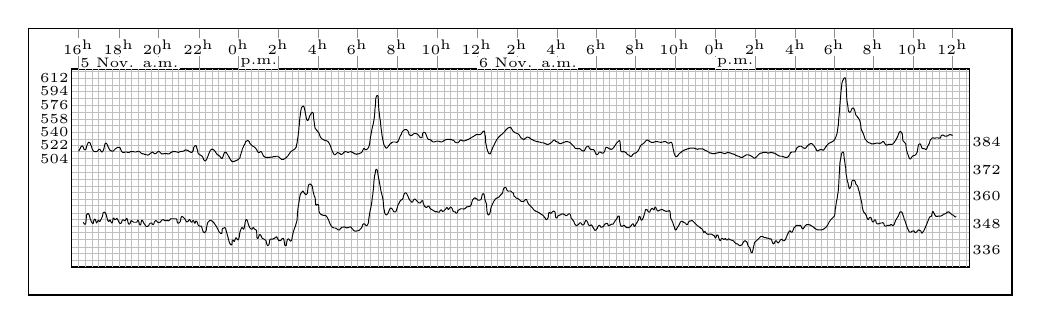
\begin{tikzpicture}[x=.049mm,y=-.049mm]
\draw[line width=.65pt] (1115,296) rectangle (3665,986);
\draw[line width=.45pt] (1227,401) rectangle (3553,914);
\begin{scope}
\clip (1227,401) rectangle (3553,914);
\draw[black!25,line width=.13pt] (1244,401) -- (1244,914);
\draw[black!25,line width=.13pt] (1261,401) -- (1261,914);
\draw[black!25,line width=.13pt] (1279,401) -- (1279,914);
\draw[black!25,line width=.13pt] (1296,401) -- (1296,914);
\draw[black!25,line width=.13pt] (1314,401) -- (1314,914);
\draw[black!25,line width=.13pt] (1331,401) -- (1331,914);
\draw[black!25,line width=.13pt] (1349,401) -- (1349,914);
\draw[black!25,line width=.13pt] (1365,401) -- (1365,914);
\draw[black!25,line width=.13pt] (1382,401) -- (1382,914);
\draw[black!25,line width=.13pt] (1400,401) -- (1400,914);
\draw[black!25,line width=.13pt] (1417,401) -- (1417,914);
\draw[black!25,line width=.13pt] (1434,401) -- (1434,914);
\draw[black!25,line width=.13pt] (1451,401) -- (1451,914);
\draw[black!25,line width=.13pt] (1468,401) -- (1468,914);
\draw[black!25,line width=.13pt] (1486,401) -- (1486,914);
\draw[black!25,line width=.13pt] (1503,401) -- (1503,914);
\draw[black!25,line width=.13pt] (1521,401) -- (1521,914);
\draw[black!25,line width=.13pt] (1539,401) -- (1539,914);
\draw[black!25,line width=.13pt] (1556,401) -- (1556,914);
\draw[black!25,line width=.13pt] (1573,401) -- (1573,914);
\draw[black!25,line width=.13pt] (1590,401) -- (1590,914);
\draw[black!25,line width=.13pt] (1607,401) -- (1607,914);
\draw[black!25,line width=.13pt] (1624,401) -- (1624,914);
\draw[black!25,line width=.13pt] (1642,401) -- (1642,914);
\draw[black!25,line width=.13pt] (1659,401) -- (1659,914);
\draw[black!25,line width=.13pt] (1676,401) -- (1676,914);
\draw[black!25,line width=.13pt] (1693,401) -- (1693,914);
\draw[black!25,line width=.13pt] (1710,401) -- (1710,914);
\draw[black!25,line width=.13pt] (1727,401) -- (1727,914);
\draw[black!25,line width=.13pt] (1744,401) -- (1744,914);
\draw[black!25,line width=.13pt] (1762,401) -- (1762,914);
\draw[black!25,line width=.13pt] (1780,401) -- (1780,914);
\draw[black!25,line width=.13pt] (1797,401) -- (1797,914);
\draw[black!25,line width=.13pt] (1814,401) -- (1814,914);
\draw[black!25,line width=.13pt] (1832,401) -- (1832,914);
\draw[black!25,line width=.13pt] (1848,401) -- (1848,914);
\draw[black!25,line width=.13pt] (1866,401) -- (1866,914);
\draw[black!25,line width=.13pt] (1883,401) -- (1883,914);
\draw[black!25,line width=.13pt] (1900,401) -- (1900,914);
\draw[black!25,line width=.13pt] (1917,401) -- (1917,914);
\draw[black!25,line width=.13pt] (1933,401) -- (1933,914);
\draw[black!25,line width=.13pt] (1950,401) -- (1950,914);
\draw[black!25,line width=.13pt] (1967,401) -- (1967,914);
\draw[black!25,line width=.13pt] (1984,401) -- (1984,914);
\draw[black!25,line width=.13pt] (2001,401) -- (2001,914);
\draw[black!25,line width=.13pt] (2021,401) -- (2021,914);
\draw[black!25,line width=.13pt] (2034,401) -- (2034,914);
\draw[black!25,line width=.13pt] (2053,401) -- (2053,914);
\draw[black!25,line width=.13pt] (2070,401) -- (2070,914);
\draw[black!25,line width=.13pt] (2087,401) -- (2087,914);
\draw[black!25,line width=.13pt] (2104,401) -- (2104,914);
\draw[black!25,line width=.13pt] (2122,401) -- (2122,914);
\draw[black!25,line width=.13pt] (2139,401) -- (2139,914);
\draw[black!25,line width=.13pt] (2156,401) -- (2156,914);
\draw[black!25,line width=.13pt] (2173,401) -- (2173,914);
\draw[black!25,line width=.13pt] (2191,401) -- (2191,914);
\draw[black!25,line width=.13pt] (2208,401) -- (2208,914);
\draw[black!25,line width=.13pt] (2225,401) -- (2225,914);
\draw[black!25,line width=.13pt] (2242,401) -- (2242,914);
\draw[black!25,line width=.13pt] (2260,401) -- (2260,914);
\draw[black!25,line width=.13pt] (2277,401) -- (2277,914);
\draw[black!25,line width=.13pt] (2295,401) -- (2295,914);
\draw[black!25,line width=.13pt] (2313,401) -- (2313,914);
\draw[black!25,line width=.13pt] (2329,401) -- (2329,914);
\draw[black!25,line width=.13pt] (2347,401) -- (2347,914);
\draw[black!25,line width=.13pt] (2364,401) -- (2364,914);
\draw[black!25,line width=.13pt] (2381,401) -- (2381,914);
\draw[black!25,line width=.13pt] (2398,401) -- (2398,914);
\draw[black!25,line width=.13pt] (2416,401) -- (2416,914);
\draw[black!25,line width=.13pt] (2433,401) -- (2433,914);
\draw[black!25,line width=.13pt] (2450,401) -- (2450,914);
\draw[black!25,line width=.13pt] (2467,401) -- (2467,914);
\draw[black!25,line width=.13pt] (2484,401) -- (2484,914);
\draw[black!25,line width=.13pt] (2501,401) -- (2501,914);
\draw[black!25,line width=.13pt] (2519,401) -- (2519,914);
\draw[black!25,line width=.13pt] (2536,401) -- (2536,914);
\draw[black!25,line width=.13pt] (2553,401) -- (2553,914);
\draw[black!25,line width=.13pt] (2570,401) -- (2570,914);
\draw[black!25,line width=.13pt] (2587,401) -- (2587,914);
\draw[black!25,line width=.13pt] (2604,401) -- (2604,914);
\draw[black!25,line width=.13pt] (2621,401) -- (2621,914);
\draw[black!25,line width=.13pt] (2638,401) -- (2638,914);
\draw[black!25,line width=.13pt] (2655,401) -- (2655,914);
\draw[black!25,line width=.13pt] (2672,401) -- (2672,914);
\draw[black!25,line width=.13pt] (2688,401) -- (2688,914);
\draw[black!25,line width=.13pt] (2703,401) -- (2703,914);
\draw[black!25,line width=.13pt] (2721,401) -- (2721,914);
\draw[black!25,line width=.13pt] (2738,401) -- (2738,914);
\draw[black!25,line width=.13pt] (2756,401) -- (2756,914);
\draw[black!25,line width=.13pt] (2773,401) -- (2773,914);
\draw[black!25,line width=.13pt] (2790,401) -- (2790,914);
\draw[black!25,line width=.13pt] (2808,401) -- (2808,914);
\draw[black!25,line width=.13pt] (2825,401) -- (2825,914);
\draw[black!25,line width=.13pt] (2842,401) -- (2842,914);
\draw[black!25,line width=.13pt] (2860,401) -- (2860,914);
\draw[black!25,line width=.13pt] (2877,401) -- (2877,914);
\draw[black!25,line width=.13pt] (2894,401) -- (2894,914);
\draw[black!25,line width=.13pt] (2911,401) -- (2911,914);
\draw[black!25,line width=.13pt] (2929,401) -- (2929,914);
\draw[black!25,line width=.13pt] (2946,401) -- (2946,914);
\draw[black!25,line width=.13pt] (2964,401) -- (2964,914);
\draw[black!25,line width=.13pt] (2981,401) -- (2981,914);
\draw[black!25,line width=.13pt] (2999,401) -- (2999,914);
\draw[black!25,line width=.13pt] (3016,401) -- (3016,914);
\draw[black!25,line width=.13pt] (3033,401) -- (3033,914);
\draw[black!25,line width=.13pt] (3051,401) -- (3051,914);
\draw[black!25,line width=.13pt] (3068,401) -- (3068,914);
\draw[black!25,line width=.13pt] (3086,401) -- (3086,914);
\draw[black!25,line width=.13pt] (3103,401) -- (3103,914);
\draw[black!25,line width=.13pt] (3121,401) -- (3121,914);
\draw[black!25,line width=.13pt] (3137,401) -- (3137,914);
\draw[black!25,line width=.13pt] (3153,401) -- (3153,914);
\draw[black!25,line width=.13pt] (3169,401) -- (3169,914);
\draw[black!25,line width=.13pt] (3186,401) -- (3186,914);
\draw[black!25,line width=.13pt] (3203,401) -- (3203,914);
\draw[black!25,line width=.13pt] (3219,401) -- (3219,914);
\draw[black!25,line width=.13pt] (3234,401) -- (3234,914);
\draw[black!25,line width=.13pt] (3253,401) -- (3253,914);
\draw[black!25,line width=.13pt] (3270,401) -- (3270,914);
\draw[black!25,line width=.13pt] (3287,401) -- (3287,914);
\draw[black!25,line width=.13pt] (3304,401) -- (3304,914);
\draw[black!25,line width=.13pt] (3321,401) -- (3321,914);
\draw[black!25,line width=.13pt] (3339,401) -- (3339,914);
\draw[black!25,line width=.13pt] (3356,401) -- (3356,914);
\draw[black!25,line width=.13pt] (3373,401) -- (3373,914);
\draw[black!25,line width=.13pt] (3389,401) -- (3389,914);
\draw[black!25,line width=.13pt] (3407,401) -- (3407,914);
\draw[black!25,line width=.13pt] (3424,401) -- (3424,914);
\draw[black!25,line width=.13pt] (3441,401) -- (3441,914);
\draw[black!25,line width=.13pt] (3458,401) -- (3458,914);
\draw[black!25,line width=.13pt] (3476,401) -- (3476,914);
\draw[black!25,line width=.13pt] (3493,401) -- (3493,914);
\draw[black!25,line width=.13pt] (3510,401) -- (3510,914);
\draw[black!25,line width=.13pt] (3528,401) -- (3528,914);
\draw[black!25,line width=.13pt] (3546,401) -- (3546,914);
\draw[black!25,line width=.13pt] (1227,407) -- (3553,407);
\draw[black!25,line width=.13pt] (1227,424) -- (3553,424);
\draw[black!25,line width=.13pt] (1227,442) -- (3553,442);
\draw[black!25,line width=.13pt] (1227,459) -- (3553,459);
\draw[black!25,line width=.13pt] (1227,477) -- (3553,477);
\draw[black!25,line width=.13pt] (1227,495) -- (3553,495);
\draw[black!25,line width=.13pt] (1227,512) -- (3553,512);
\draw[black!25,line width=.13pt] (1227,530) -- (3553,530);
\draw[black!25,line width=.13pt] (1227,547) -- (3553,547);
\draw[black!25,line width=.13pt] (1227,564) -- (3553,564);
\draw[black!25,line width=.13pt] (1227,582) -- (3553,582);
\draw[black!25,line width=.13pt] (1227,598) -- (3553,598);
\draw[black!25,line width=.13pt] (1227,615) -- (3553,615);
\draw[black!25,line width=.13pt] (1227,633) -- (3553,633);
\draw[black!25,line width=.13pt] (1227,651) -- (3553,651);
\draw[black!25,line width=.13pt] (1227,669) -- (3553,669);
\draw[black!25,line width=.13pt] (1227,686) -- (3553,686);
\draw[black!25,line width=.13pt] (1227,704) -- (3553,704);
\draw[black!25,line width=.13pt] (1227,721) -- (3553,721);
\draw[black!25,line width=.13pt] (1227,738) -- (3553,738);
\draw[black!25,line width=.13pt] (1227,755) -- (3553,755);
\draw[black!25,line width=.13pt] (1227,774) -- (3553,774);
\draw[black!25,line width=.13pt] (1227,790) -- (3553,790);
\draw[black!25,line width=.13pt] (1227,808) -- (3553,808);
\draw[black!25,line width=.13pt] (1227,825) -- (3553,825);
\draw[black!25,line width=.13pt] (1227,843) -- (3553,843);
\draw[black!25,line width=.13pt] (1227,862) -- (3553,862);
\draw[black!25,line width=.13pt] (1227,878) -- (3553,878);
\draw[black!25,line width=.13pt] (1227,896) -- (3553,896);
\end{scope}
\draw[black!45,line width=.15pt] (1244,296) -- (1244,401);
\node[font=\tiny,fill=white,inner sep=.4pt] at (1244,344) {$16^{\mathrm{h}}$};
\draw[black!45,line width=.15pt] (1349,296) -- (1349,401);
\node[font=\tiny,fill=white,inner sep=.4pt] at (1349,344) {$18^{\mathrm{h}}$};
\draw[black!45,line width=.15pt] (1451,296) -- (1451,401);
\node[font=\tiny,fill=white,inner sep=.4pt] at (1451,344) {$20^{\mathrm{h}}$};
\draw[black!45,line width=.15pt] (1556,296) -- (1556,401);
\node[font=\tiny,fill=white,inner sep=.4pt] at (1556,344) {$22^{\mathrm{h}}$};
\draw[black!45,line width=.15pt] (1659,296) -- (1659,401);
\node[font=\tiny,fill=white,inner sep=.4pt] at (1659,344) {$0^{\mathrm{h}}$};
\draw[black!45,line width=.15pt] (1762,296) -- (1762,401);
\node[font=\tiny,fill=white,inner sep=.4pt] at (1762,344) {$2^{\mathrm{h}}$};
\draw[black!45,line width=.15pt] (1866,296) -- (1866,401);
\node[font=\tiny,fill=white,inner sep=.4pt] at (1866,344) {$4^{\mathrm{h}}$};
\draw[black!45,line width=.15pt] (1967,296) -- (1967,401);
\node[font=\tiny,fill=white,inner sep=.4pt] at (1967,344) {$6^{\mathrm{h}}$};
\draw[black!45,line width=.15pt] (2070,296) -- (2070,401);
\node[font=\tiny,fill=white,inner sep=.4pt] at (2070,344) {$8^{\mathrm{h}}$};
\draw[black!45,line width=.15pt] (2173,296) -- (2173,401);
\node[font=\tiny,fill=white,inner sep=.4pt] at (2173,344) {$10^{\mathrm{h}}$};
\draw[black!45,line width=.15pt] (2277,296) -- (2277,401);
\node[font=\tiny,fill=white,inner sep=.4pt] at (2277,344) {$12^{\mathrm{h}}$};
\draw[black!45,line width=.15pt] (2381,296) -- (2381,401);
\node[font=\tiny,fill=white,inner sep=.4pt] at (2381,344) {$2^{\mathrm{h}}$};
\draw[black!45,line width=.15pt] (2484,296) -- (2484,401);
\node[font=\tiny,fill=white,inner sep=.4pt] at (2484,344) {$4^{\mathrm{h}}$};
\draw[black!45,line width=.15pt] (2587,296) -- (2587,401);
\node[font=\tiny,fill=white,inner sep=.4pt] at (2587,344) {$6^{\mathrm{h}}$};
\draw[black!45,line width=.15pt] (2688,296) -- (2688,401);
\node[font=\tiny,fill=white,inner sep=.4pt] at (2688,344) {$8^{\mathrm{h}}$};
\draw[black!45,line width=.15pt] (2790,296) -- (2790,401);
\node[font=\tiny,fill=white,inner sep=.4pt] at (2790,344) {$10^{\mathrm{h}}$};
\draw[black!45,line width=.15pt] (2894,296) -- (2894,401);
\node[font=\tiny,fill=white,inner sep=.4pt] at (2894,344) {$0^{\mathrm{h}}$};
\draw[black!45,line width=.15pt] (2999,296) -- (2999,401);
\node[font=\tiny,fill=white,inner sep=.4pt] at (2999,344) {$2^{\mathrm{h}}$};
\draw[black!45,line width=.15pt] (3103,296) -- (3103,401);
\node[font=\tiny,fill=white,inner sep=.4pt] at (3103,344) {$4^{\mathrm{h}}$};
\draw[black!45,line width=.15pt] (3203,296) -- (3203,401);
\node[font=\tiny,fill=white,inner sep=.4pt] at (3203,344) {$6^{\mathrm{h}}$};
\draw[black!45,line width=.15pt] (3304,296) -- (3304,401);
\node[font=\tiny,fill=white,inner sep=.4pt] at (3304,344) {$8^{\mathrm{h}}$};
\draw[black!45,line width=.15pt] (3407,296) -- (3407,401);
\node[font=\tiny,fill=white,inner sep=.4pt] at (3407,344) {$10^{\mathrm{h}}$};
\draw[black!45,line width=.15pt] (3510,296) -- (3510,401);
\node[font=\tiny,fill=white,inner sep=.4pt] at (3510,344) {$12^{\mathrm{h}}$};
\node[anchor=east,font=\tiny,inner sep=1pt] at (1227,424) {612};
\node[anchor=east,font=\tiny,inner sep=1pt] at (1227,459) {594};
\node[anchor=east,font=\tiny,inner sep=1pt] at (1227,495) {576};
\node[anchor=east,font=\tiny,inner sep=1pt] at (1227,530) {558};
\node[anchor=east,font=\tiny,inner sep=1pt] at (1227,564) {540};
\node[anchor=east,font=\tiny,inner sep=1pt] at (1227,598) {522};
\node[anchor=east,font=\tiny,inner sep=1pt] at (1227,633) {504};
\node[anchor=west,font=\tiny,inner sep=1pt] at (3553,591) {384};
\node[anchor=west,font=\tiny,inner sep=1pt] at (3553,662) {372};
\node[anchor=west,font=\tiny,inner sep=1pt] at (3553,731) {360};
\node[anchor=west,font=\tiny,inner sep=1pt] at (3553,802) {348};
\node[anchor=west,font=\tiny,inner sep=1pt] at (3553,871) {336};
% upper_copenhagen: trace of visible engraved ink in image coordinates.
\draw[line width=.34pt,line join=round] plot coordinates {
  (1244,613) (1245,613) (1246,612) (1247,610) (1248,608) (1249,606) (1250,604) (1251,602) (1252,601)
  (1253,600) (1254,600) (1255,601) (1256,602) (1257,604) (1258,607) (1259,609) (1260,610) (1261,610)
  (1262,610) (1263,609) (1264,608) (1265,604) (1266,600) (1267,597) (1268,595) (1269,593) (1270,591)
  (1271,591) (1272,591) (1273,591) (1274,592) (1275,594) (1276,597) (1277,599) (1278,602) (1279,605)
  (1280,608) (1281,610) (1282,612) (1283,613) (1284,614) (1285,615) (1286,615) (1287,615) (1288,615)
  (1289,615) (1290,615) (1291,615) (1292,615) (1293,614) (1294,613) (1295,612) (1296,611) (1297,609)
  (1298,609) (1299,609) (1300,609) (1301,611) (1302,613) (1303,614) (1304,615) (1305,616) (1306,616)
  (1307,615) (1308,613) (1309,611) (1310,608) (1311,604) (1312,599) (1313,595) (1314,594) (1315,593)
  (1316,593) (1317,594) (1318,595) (1319,597) (1320,600) (1321,602) (1322,604) (1323,606) (1324,608)
  (1325,610) (1326,611) (1327,612) (1328,612) (1329,613) (1330,613) (1331,614) (1332,614) (1333,614)
  (1334,614) (1335,613) (1336,612) (1337,611) (1338,610) (1339,609) (1340,608) (1341,607) (1342,606)
  (1343,606) (1344,605) (1345,604) (1346,604) (1347,604) (1348,604) (1349,604) (1350,604) (1351,604)
  (1352,605) (1353,607) (1354,610) (1355,612) (1356,614) (1357,615) (1358,616) (1359,617) (1360,617)
  (1361,617) (1362,617) (1363,617) (1364,617) (1365,616) (1366,616) (1367,616) (1368,616) (1369,616)
  (1370,616) (1371,617) (1372,617) (1373,617) (1374,617) (1375,617) (1376,617) (1377,616) (1378,616)
  (1379,615) (1380,615) (1381,615) (1382,615) (1383,615) (1384,615) (1385,615) (1386,615) (1387,615)
  (1388,615) (1389,616) (1390,616) (1391,616) (1392,616) (1393,616) (1394,616) (1395,615) (1396,615)
  (1397,615) (1398,614) (1399,614) (1400,614) (1401,614) (1402,615) (1403,615) (1404,616) (1405,617)
  (1406,618) (1407,619) (1408,620) (1409,620) (1410,620) (1411,621) (1412,621) (1413,621) (1414,621)
  (1415,622) (1416,622) (1417,622) (1418,622) (1419,623) (1420,623) (1421,623) (1422,623) (1423,624)
  (1424,624) (1425,624) (1426,623) (1427,623) (1428,622) (1429,621) (1430,620) (1431,619) (1432,619)
  (1433,618) (1434,617) (1435,616) (1436,616) (1437,617) (1438,617) (1439,618) (1440,619) (1441,620)
  (1442,620) (1443,620) (1444,620) (1445,620) (1446,619) (1447,618) (1448,617) (1449,616) (1450,615)
  (1451,614) (1452,614) (1453,614) (1454,615) (1455,616) (1456,617) (1457,618) (1458,619) (1459,620)
  (1460,620) (1461,621) (1462,621) (1463,621) (1464,621) (1465,621) (1466,620) (1467,620) (1468,620)
  (1469,620) (1470,620) (1471,620) (1472,620) (1473,620) (1474,620) (1475,621) (1476,621) (1477,621)
  (1478,621) (1479,621) (1480,620) (1481,619) (1482,619) (1483,618) (1484,617) (1485,617) (1486,616)
  (1487,616) (1488,615) (1489,615) (1490,615) (1491,615) (1492,614) (1493,615) (1494,615) (1495,615)
  (1496,615) (1497,615) (1498,616) (1499,616) (1500,616) (1501,616) (1502,617) (1503,617) (1504,617)
  (1505,616) (1506,616) (1507,615) (1508,615) (1509,615) (1510,615) (1511,614) (1512,614) (1513,615)
  (1514,614) (1515,614) (1516,614) (1517,613) (1518,613) (1519,612) (1520,611) (1521,611) (1522,611)
  (1523,610) (1524,611) (1525,611) (1526,611) (1527,612) (1528,612) (1529,613) (1530,613) (1531,614)
  (1532,615) (1533,615) (1534,616) (1535,616) (1536,617) (1537,617) (1538,617) (1539,616) (1540,615)
  (1541,613) (1542,611) (1543,605) (1544,603) (1545,601) (1546,600) (1547,600) (1548,599) (1549,600)
  (1550,601) (1551,605) (1552,609) (1553,611) (1554,618) (1555,620) (1556,621) (1557,622) (1558,623)
  (1559,623) (1560,624) (1561,624) (1562,625) (1563,626) (1564,626) (1565,627) (1566,629) (1567,630)
  (1568,633) (1569,636) (1570,637) (1571,638) (1572,639) (1573,639) (1574,638) (1575,637) (1576,636)
  (1577,634) (1578,631) (1579,629) (1580,626) (1581,624) (1582,621) (1583,619) (1584,616) (1585,614)
  (1586,612) (1587,611) (1588,610) (1589,609) (1590,609) (1591,608) (1592,609) (1593,609) (1594,610)
  (1595,611) (1596,611) (1597,612) (1598,614) (1599,615) (1600,617) (1601,618) (1602,620) (1603,621)
  (1604,622) (1605,623) (1606,624) (1607,624) (1608,625) (1609,626) (1610,626) (1611,627) (1612,629)
  (1613,630) (1614,632) (1615,632) (1616,633) (1617,632) (1618,630) (1619,628) (1620,625) (1621,622)
  (1622,619) (1623,617) (1624,617) (1625,616) (1626,617) (1627,617) (1628,618) (1629,620) (1630,621)
  (1631,623) (1632,625) (1633,627) (1634,628) (1635,630) (1636,632) (1637,634) (1638,635) (1639,637)
  (1640,638) (1641,639) (1642,640) (1643,641) (1644,641) (1645,641) (1646,641) (1647,640) (1648,640)
  (1649,640) (1650,639) (1651,639) (1652,639) (1653,638) (1654,638) (1655,637) (1656,637) (1657,636)
  (1658,635) (1659,635) (1660,634) (1661,633) (1662,632) (1663,631) (1664,624) (1665,623) (1666,619)
  (1667,616) (1668,613) (1669,608) (1670,606) (1671,604) (1672,602) (1673,599) (1674,598) (1675,596)
  (1676,594) (1677,591) (1678,589) (1679,588) (1680,588) (1681,587) (1682,586) (1683,586) (1684,587)
  (1685,587) (1686,588) (1687,589) (1688,592) (1689,594) (1690,595) (1691,596) (1692,597) (1693,598)
  (1694,599) (1695,600) (1696,601) (1697,601) (1698,602) (1699,602) (1700,603) (1701,604) (1702,604)
  (1703,606) (1704,607) (1705,608) (1706,610) (1707,611) (1708,614) (1709,615) (1710,617) (1711,617)
  (1712,618) (1713,617) (1714,617) (1715,616) (1716,615) (1717,615) (1718,615) (1719,616) (1720,618)
  (1721,620) (1722,622) (1723,625) (1724,626) (1725,627) (1726,628) (1727,629) (1728,629) (1729,629)
  (1730,630) (1731,630) (1732,630) (1733,630) (1734,630) (1735,630) (1736,630) (1737,630) (1738,630)
  (1739,630) (1740,630) (1741,629) (1742,629) (1743,629) (1744,629) (1745,629) (1746,629) (1747,629)
  (1748,629) (1749,628) (1750,628) (1751,628) (1752,628) (1753,628) (1754,628) (1755,628) (1756,627)
  (1757,627) (1758,627) (1759,627) (1760,627) (1761,627) (1762,628) (1763,629) (1764,629) (1765,630)
  (1766,631) (1767,632) (1768,633) (1769,634) (1770,634) (1771,635) (1772,635) (1773,635) (1774,635)
  (1775,635) (1776,635) (1777,634) (1778,634) (1779,633) (1780,632) (1781,632) (1782,631) (1783,630)
  (1784,630) (1785,628) (1786,627) (1787,626) (1788,625) (1789,623) (1790,622) (1791,620) (1792,619)
  (1793,617) (1794,616) (1795,615) (1796,614) (1797,613) (1798,613) (1799,612) (1800,612) (1801,611)
  (1802,610) (1803,610) (1804,609) (1805,608) (1806,607) (1807,606) (1808,604) (1809,602) (1810,596)
  (1811,592) (1812,584) (1813,579) (1814,571) (1815,563) (1816,551) (1817,543) (1818,528) (1819,523)
  (1820,514) (1821,508) (1822,503) (1823,500) (1824,499) (1825,498) (1826,497) (1827,497) (1828,498)
  (1829,499) (1830,503) (1831,508) (1832,512) (1833,519) (1834,523) (1835,528) (1836,532) (1837,533)
  (1838,534) (1839,534) (1840,533) (1841,530) (1842,528) (1843,525) (1844,522) (1845,520) (1846,519)
  (1847,517) (1848,516) (1849,514) (1850,514) (1851,513) (1852,514) (1853,516) (1854,530) (1855,536)
  (1856,544) (1857,551) (1858,555) (1859,556) (1860,557) (1861,559) (1862,560) (1863,561) (1864,562)
  (1865,563) (1866,565) (1867,566) (1868,568) (1869,570) (1870,574) (1871,576) (1872,578) (1873,579)
  (1874,580) (1875,581) (1876,582) (1877,583) (1878,583) (1879,584) (1880,584) (1881,585) (1882,585)
  (1883,586) (1884,586) (1885,586) (1886,586) (1887,587) (1888,587) (1889,588) (1890,588) (1891,589)
  (1892,590) (1893,592) (1894,593) (1895,595) (1896,597) (1897,599) (1898,602) (1899,605) (1900,608)
  (1901,610) (1902,613) (1903,615) (1904,617) (1905,619) (1906,621) (1907,622) (1908,623) (1909,623)
  (1910,623) (1911,622) (1912,621) (1913,620) (1914,619) (1915,618) (1916,617) (1917,617) (1918,618)
  (1919,618) (1920,619) (1921,620) (1922,620) (1923,621) (1924,622) (1925,622) (1926,622) (1927,622)
  (1928,621) (1929,621) (1930,620) (1931,619) (1932,617) (1933,617) (1934,616) (1935,615) (1936,615)
  (1937,615) (1938,615) (1939,616) (1940,616) (1941,616) (1942,617) (1943,617) (1944,617) (1945,616)
  (1946,616) (1947,616) (1948,616) (1949,615) (1950,615) (1951,615) (1952,616) (1953,616) (1954,617)
  (1955,617) (1956,618) (1957,618) (1958,619) (1959,620) (1960,620) (1961,621) (1962,621) (1963,621)
  (1964,621) (1965,622) (1966,622) (1967,621) (1968,621) (1969,621) (1970,621) (1971,621) (1972,620)
  (1973,620) (1974,619) (1975,619) (1976,618) (1977,618) (1978,617) (1979,616) (1980,615) (1981,612)
  (1982,610) (1983,608) (1984,607) (1985,607) (1986,607) (1987,609) (1988,610) (1989,610) (1990,610)
  (1991,610) (1992,609) (1993,608) (1994,607) (1995,606) (1996,604) (1997,602) (1998,599) (1999,594)
  (2000,587) (2001,579) (2002,574) (2003,568) (2004,564) (2005,557) (2006,552) (2007,548) (2008,545)
  (2009,539) (2010,534) (2011,528) (2012,519) (2013,503) (2014,496) (2015,476) (2016,474) (2017,471)
  (2018,470) (2019,470) (2020,470) (2021,471) (2022,490) (2023,508) (2024,514) (2025,524) (2026,531)
  (2027,536) (2028,548) (2029,556) (2030,563) (2031,572) (2032,577) (2033,583) (2034,587) (2035,593)
  (2036,597) (2037,599) (2038,601) (2039,602) (2040,604) (2041,605) (2042,606) (2043,606) (2044,605)
  (2045,604) (2046,603) (2047,602) (2048,600) (2049,599) (2050,598) (2051,596) (2052,595) (2053,594)
  (2054,594) (2055,593) (2056,592) (2057,591) (2058,591) (2059,590) (2060,590) (2061,590) (2062,590)
  (2063,590) (2064,590) (2065,590) (2066,590) (2067,590) (2068,591) (2069,591) (2070,591) (2071,590)
  (2072,589) (2073,588) (2074,586) (2075,583) (2076,581) (2077,578) (2078,575) (2079,574) (2080,572)
  (2081,570) (2082,567) (2083,565) (2084,563) (2085,562) (2086,561) (2087,560) (2088,559) (2089,559)
  (2090,558) (2091,558) (2092,558) (2093,558) (2094,558) (2095,558) (2096,559) (2097,560) (2098,561)
  (2099,563) (2100,565) (2101,570) (2102,571) (2103,572) (2104,573) (2105,573) (2106,573) (2107,573)
  (2108,573) (2109,572) (2110,572) (2111,570) (2112,570) (2113,569) (2114,568) (2115,568) (2116,568)
  (2117,568) (2118,568) (2119,568) (2120,569) (2121,569) (2122,569) (2123,570) (2124,571) (2125,572)
  (2126,573) (2127,574) (2128,576) (2129,577) (2130,578) (2131,578) (2132,579) (2133,579) (2134,579)
  (2135,578) (2136,570) (2137,567) (2138,566) (2139,565) (2140,565) (2141,565) (2142,565) (2143,566)
  (2144,568) (2145,570) (2146,572) (2147,575) (2148,578) (2149,580) (2150,582) (2151,583) (2152,583)
  (2153,583) (2154,584) (2155,584) (2156,584) (2157,585) (2158,585) (2159,586) (2160,587) (2161,588)
  (2162,589) (2163,589) (2164,590) (2165,590) (2166,590) (2167,590) (2168,589) (2169,589) (2170,589)
  (2171,588) (2172,588) (2173,588) (2174,588) (2175,587) (2176,588) (2177,588) (2178,588) (2179,588)
  (2180,589) (2181,589) (2182,589) (2183,590) (2184,590) (2185,590) (2186,590) (2187,589) (2188,589)
  (2189,588) (2190,588) (2191,587) (2192,586) (2193,586) (2194,585) (2195,585) (2196,584) (2197,584)
  (2198,584) (2199,583) (2200,583) (2201,583) (2202,583) (2203,583) (2204,583) (2205,583) (2206,583)
  (2207,583) (2208,583) (2209,583) (2210,584) (2211,584) (2212,584) (2213,585) (2214,585) (2215,585)
  (2216,586) (2217,586) (2218,587) (2219,589) (2220,590) (2221,590) (2222,591) (2223,591) (2224,592)
  (2225,592) (2226,592) (2227,592) (2228,592) (2229,591) (2230,590) (2231,589) (2232,588) (2233,586)
  (2234,585) (2235,585) (2236,585) (2237,585) (2238,586) (2239,586) (2240,587) (2241,587) (2242,587)
  (2243,587) (2244,587) (2245,587) (2246,587) (2247,586) (2248,586) (2249,586) (2250,585) (2251,585)
  (2252,584) (2253,584) (2254,584) (2255,583) (2256,583) (2257,582) (2258,581) (2259,581) (2260,580)
  (2261,580) (2262,579) (2263,579) (2264,578) (2265,577) (2266,577) (2267,576) (2268,576) (2269,575)
  (2270,574) (2271,574) (2272,573) (2273,572) (2274,572) (2275,571) (2276,571) (2277,570) (2278,570)
  (2279,570) (2280,571) (2281,571) (2282,571) (2283,571) (2284,571) (2285,571) (2286,570) (2287,570)
  (2288,569) (2289,568) (2290,567) (2291,565) (2292,564) (2293,563) (2294,562) (2295,562) (2296,562)
  (2297,563) (2298,572) (2299,575) (2300,593) (2301,597) (2302,602) (2303,607) (2304,610) (2305,613)
  (2306,616) (2307,618) (2308,619) (2309,620) (2310,620) (2311,621) (2312,620) (2313,618) (2314,615)
  (2315,612) (2316,610) (2317,608) (2318,605) (2319,603) (2320,601) (2321,599) (2322,597) (2323,595)
  (2324,592) (2325,591) (2326,589) (2327,587) (2328,585) (2329,583) (2330,582) (2331,581) (2332,579)
  (2333,578) (2334,577) (2335,576) (2336,575) (2337,574) (2338,573) (2339,572) (2340,571) (2341,571)
  (2342,570) (2343,569) (2344,568) (2345,567) (2346,566) (2347,565) (2348,564) (2349,563) (2350,562)
  (2351,560) (2352,559) (2353,558) (2354,557) (2355,556) (2356,555) (2357,554) (2358,554) (2359,553)
  (2360,553) (2361,552) (2362,552) (2363,552) (2364,552) (2365,553) (2366,554) (2367,556) (2368,557)
  (2369,559) (2370,561) (2371,562) (2372,563) (2373,564) (2374,564) (2375,565) (2376,566) (2377,566)
  (2378,567) (2379,567) (2380,567) (2381,568) (2382,568) (2383,568) (2384,569) (2385,570) (2386,571)
  (2387,572) (2388,574) (2389,576) (2390,577) (2391,579) (2392,580) (2393,580) (2394,581) (2395,582)
  (2396,582) (2397,583) (2398,583) (2399,583) (2400,583) (2401,582) (2402,581) (2403,580) (2404,580)
  (2405,579) (2406,578) (2407,577) (2408,577) (2409,577) (2410,578) (2411,578) (2412,578) (2413,579)
  (2414,580) (2415,580) (2416,581) (2417,582) (2418,583) (2419,583) (2420,584) (2421,584) (2422,585)
  (2423,585) (2424,586) (2425,586) (2426,587) (2427,587) (2428,587) (2429,588) (2430,588) (2431,588)
  (2432,589) (2433,589) (2434,589) (2435,589) (2436,589) (2437,590) (2438,590) (2439,590) (2440,590)
  (2441,591) (2442,591) (2443,591) (2444,592) (2445,592) (2446,592) (2447,592) (2448,592) (2449,592)
  (2450,592) (2451,593) (2452,593) (2453,594) (2454,594) (2455,595) (2456,595) (2457,595) (2458,596)
  (2459,596) (2460,596) (2461,596) (2462,596) (2463,596) (2464,595) (2465,595) (2466,594) (2467,594)
  (2468,593) (2469,592) (2470,591) (2471,590) (2472,590) (2473,588) (2474,587) (2475,586) (2476,586)
  (2477,585) (2478,585) (2479,585) (2480,586) (2481,588) (2482,589) (2483,589) (2484,589) (2485,590)
  (2486,590) (2487,590) (2488,591) (2489,592) (2490,593) (2491,594) (2492,594) (2493,594) (2494,594)
  (2495,594) (2496,594) (2497,593) (2498,593) (2499,592) (2500,592) (2501,591) (2502,591) (2503,591)
  (2504,590) (2505,590) (2506,590) (2507,589) (2508,589) (2509,589) (2510,589) (2511,589) (2512,589)
  (2513,589) (2514,590) (2515,590) (2516,590) (2517,591) (2518,591) (2519,592) (2520,593) (2521,594)
  (2522,595) (2523,596) (2524,597) (2525,598) (2526,599) (2527,600) (2528,601) (2529,602) (2530,604)
  (2531,605) (2532,606) (2533,607) (2534,607) (2535,607) (2536,607) (2537,607) (2538,607) (2539,607)
  (2540,607) (2541,607) (2542,607) (2543,607) (2544,608) (2545,608) (2546,609) (2547,610) (2548,611)
  (2549,612) (2550,612) (2551,613) (2552,613) (2553,613) (2554,614) (2555,613) (2556,612) (2557,610)
  (2558,608) (2559,606) (2560,604) (2561,603) (2562,602) (2563,601) (2564,601) (2565,601) (2566,601)
  (2567,602) (2568,605) (2569,607) (2570,608) (2571,608) (2572,609) (2573,609) (2574,609) (2575,610)
  (2576,610) (2577,610) (2578,610) (2579,610) (2580,610) (2581,611) (2582,613) (2583,615) (2584,618)
  (2585,620) (2586,622) (2587,622) (2588,623) (2589,623) (2590,622) (2591,621) (2592,620) (2593,618)
  (2594,617) (2595,616) (2596,616) (2597,616) (2598,617) (2599,617) (2600,618) (2601,619) (2602,619)
  (2603,619) (2604,619) (2605,618) (2606,617) (2607,616) (2608,614) (2609,612) (2610,607) (2611,605)
  (2612,604) (2613,604) (2614,604) (2615,604) (2616,605) (2617,605) (2618,606) (2619,607) (2620,607)
  (2621,608) (2622,608) (2623,608) (2624,609) (2625,609) (2626,609) (2627,608) (2628,608) (2629,607)
  (2630,606) (2631,605) (2632,604) (2633,602) (2634,601) (2635,599) (2636,598) (2637,596) (2638,595)
  (2639,593) (2640,592) (2641,591) (2642,590) (2643,589) (2644,588) (2645,587) (2646,586) (2647,587)
  (2648,589) (2649,599) (2650,613) (2651,614) (2652,615) (2653,615) (2654,616) (2655,615) (2656,615)
  (2657,614) (2658,615) (2659,615) (2660,616) (2661,616) (2662,617) (2663,617) (2664,618) (2665,619)
  (2666,621) (2667,622) (2668,623) (2669,623) (2670,624) (2671,624) (2672,624) (2673,626) (2674,626)
  (2675,627) (2676,628) (2677,627) (2678,627) (2679,626) (2680,624) (2681,622) (2682,622) (2683,621)
  (2684,620) (2685,619) (2686,619) (2687,619) (2688,619) (2689,618) (2690,618) (2691,617) (2692,616)
  (2693,615) (2694,614) (2695,612) (2696,611) (2697,609) (2698,607) (2699,605) (2700,602) (2701,600)
  (2702,599) (2703,598) (2704,597) (2705,596) (2706,596) (2707,595) (2708,594) (2709,593) (2710,593)
  (2711,592) (2712,591) (2713,589) (2714,588) (2715,587) (2716,586) (2717,586) (2718,585) (2719,585)
  (2720,585) (2721,586) (2722,586) (2723,587) (2724,588) (2725,589) (2726,589) (2727,590) (2728,590)
  (2729,591) (2730,591) (2731,591) (2732,591) (2733,591) (2734,591) (2735,591) (2736,590) (2737,590)
  (2738,590) (2739,589) (2740,589) (2741,589) (2742,589) (2743,589) (2744,589) (2745,589) (2746,589)
  (2747,590) (2748,590) (2749,590) (2750,590) (2751,590) (2752,591) (2753,591) (2754,591) (2755,591)
  (2756,591) (2757,590) (2758,590) (2759,590) (2760,590) (2761,589) (2762,589) (2763,589) (2764,589)
  (2765,589) (2766,589) (2767,589) (2768,590) (2769,591) (2770,592) (2771,592) (2772,593) (2773,593)
  (2774,593) (2775,593) (2776,593) (2777,592) (2778,591) (2779,591) (2780,591) (2781,591) (2782,592)
  (2783,594) (2784,598) (2785,603) (2786,609) (2787,613) (2788,619) (2789,621) (2790,623) (2791,626)
  (2792,627) (2793,628) (2794,628) (2795,628) (2796,627) (2797,626) (2798,625) (2799,624) (2800,622)
  (2801,621) (2802,620) (2803,619) (2804,618) (2805,618) (2806,617) (2807,616) (2808,615) (2809,614)
  (2810,614) (2811,613) (2812,612) (2813,612) (2814,611) (2815,611) (2816,611) (2817,610) (2818,610)
  (2819,610) (2820,609) (2821,609) (2822,608) (2823,608) (2824,608) (2825,607) (2826,607) (2827,607)
  (2828,607) (2829,606) (2830,606) (2831,606) (2832,606) (2833,606) (2834,606) (2835,606) (2836,606)
  (2837,606) (2838,606) (2839,606) (2840,606) (2841,606) (2842,607) (2843,607) (2844,608) (2845,608)
  (2846,608) (2847,608) (2848,609) (2849,609) (2850,609) (2851,608) (2852,608) (2853,608) (2854,608)
  (2855,608) (2856,608) (2857,608) (2858,608) (2859,608) (2860,608) (2861,608) (2862,608) (2863,608)
  (2864,609) (2865,609) (2866,610) (2867,611) (2868,611) (2869,612) (2870,612) (2871,613) (2872,613)
  (2873,613) (2874,614) (2875,614) (2876,615) (2877,616) (2878,616) (2879,617) (2880,618) (2881,618)
  (2882,619) (2883,619) (2884,619) (2885,619) (2886,620) (2887,620) (2888,620) (2889,620) (2890,620)
  (2891,620) (2892,620) (2893,620) (2894,620) (2895,620) (2896,619) (2897,619) (2898,619) (2899,619)
  (2900,618) (2901,618) (2902,618) (2903,618) (2904,617) (2905,617) (2906,617) (2907,617) (2908,617)
  (2909,617) (2910,617) (2911,617) (2912,618) (2913,618) (2914,618) (2915,619) (2916,619) (2917,620)
  (2918,620) (2919,620) (2920,620) (2921,620) (2922,619) (2923,619) (2924,618) (2925,618) (2926,618)
  (2927,617) (2928,617) (2929,617) (2930,617) (2931,618) (2932,618) (2933,618) (2934,619) (2935,619)
  (2936,619) (2937,620) (2938,620) (2939,621) (2940,621) (2941,621) (2942,621) (2943,622) (2944,622)
  (2945,622) (2946,623) (2947,624) (2948,624) (2949,625) (2950,625) (2951,626) (2952,626) (2953,626)
  (2954,627) (2955,627) (2956,627) (2957,628) (2958,628) (2959,629) (2960,629) (2961,630) (2962,630)
  (2963,630) (2964,630) (2965,630) (2966,629) (2967,629) (2968,628) (2969,627) (2970,627) (2971,626)
  (2972,626) (2973,625) (2974,624) (2975,624) (2976,623) (2977,623) (2978,623) (2979,623) (2980,623)
  (2981,623) (2982,624) (2983,624) (2984,624) (2985,625) (2986,625) (2987,626) (2988,626) (2989,627)
  (2990,628) (2991,628) (2992,629) (2993,630) (2994,631) (2995,631) (2996,632) (2997,632) (2998,632)
  (2999,631) (3000,630) (3001,629) (3002,629) (3003,627) (3004,626) (3005,625) (3006,624) (3007,623)
  (3008,622) (3009,621) (3010,620) (3011,620) (3012,619) (3013,619) (3014,619) (3015,619) (3016,618)
  (3017,618) (3018,617) (3019,617) (3020,617) (3021,617) (3022,617) (3023,617) (3024,617) (3025,617)
  (3026,617) (3027,617) (3028,617) (3029,618) (3030,618) (3031,619) (3032,619) (3033,618) (3034,618)
  (3035,618) (3036,618) (3037,618) (3038,617) (3039,617) (3040,617) (3041,617) (3042,617) (3043,618)
  (3044,618) (3045,618) (3046,619) (3047,619) (3048,619) (3049,619) (3050,620) (3051,620) (3052,621)
  (3053,622) (3054,622) (3055,623) (3056,624) (3057,624) (3058,625) (3059,625) (3060,626) (3061,626)
  (3062,626) (3063,627) (3064,627) (3065,627) (3066,627) (3067,627) (3068,627) (3069,627) (3070,628)
  (3071,628) (3072,628) (3073,629) (3074,629) (3075,629) (3076,630) (3077,630) (3078,630) (3079,630)
  (3080,630) (3081,630) (3082,629) (3083,629) (3084,628) (3085,627) (3086,625) (3087,624) (3088,622)
  (3089,620) (3090,618) (3091,617) (3092,617) (3093,616) (3094,616) (3095,616) (3096,616) (3097,616)
  (3098,616) (3099,616) (3100,616) (3101,616) (3102,615) (3103,613) (3104,611) (3105,608) (3106,606)
  (3107,605) (3108,604) (3109,603) (3110,603) (3111,602) (3112,602) (3113,601) (3114,601) (3115,601)
  (3116,601) (3117,601) (3118,601) (3119,602) (3120,603) (3121,603) (3122,604) (3123,605) (3124,606)
  (3125,606) (3126,606) (3127,607) (3128,606) (3129,606) (3130,605) (3131,604) (3132,602) (3133,601)
  (3134,600) (3135,599) (3136,598) (3137,597) (3138,597) (3139,596) (3140,595) (3141,595) (3142,594)
  (3143,594) (3144,594) (3145,594) (3146,595) (3147,596) (3148,597) (3149,598) (3150,599) (3151,600)
  (3152,602) (3153,603) (3154,605) (3155,606) (3156,608) (3157,610) (3158,612) (3159,613) (3160,613)
  (3161,613) (3162,612) (3163,612) (3164,611) (3165,611) (3166,610) (3167,610) (3168,610) (3169,610)
  (3170,610) (3171,610) (3172,610) (3173,611) (3174,611) (3175,611) (3176,611) (3177,609) (3178,608)
  (3179,606) (3180,605) (3181,603) (3182,602) (3183,601) (3184,599) (3185,598) (3186,597) (3187,596)
  (3188,595) (3189,594) (3190,593) (3191,593) (3192,592) (3193,592) (3194,591) (3195,591) (3196,590)
  (3197,590) (3198,589) (3199,589) (3200,588) (3201,587) (3202,587) (3203,585) (3204,584) (3205,583)
  (3206,580) (3207,578) (3208,576) (3209,572) (3210,570) (3211,566) (3212,559) (3213,551) (3214,546)
  (3215,529) (3216,520) (3217,507) (3218,495) (3219,481) (3220,471) (3221,458) (3222,450) (3223,439)
  (3224,435) (3225,432) (3226,430) (3227,428) (3228,426) (3229,424) (3230,424) (3231,424) (3232,424)
  (3233,426) (3234,441) (3235,460) (3236,480) (3237,487) (3238,493) (3239,500) (3240,509) (3241,511)
  (3242,512) (3243,513) (3244,513) (3245,512) (3246,511) (3247,509) (3248,506) (3249,504) (3250,503)
  (3251,502) (3252,502) (3253,502) (3254,503) (3255,505) (3256,507) (3257,511) (3258,515) (3259,519)
  (3260,521) (3261,522) (3262,523) (3263,524) (3264,526) (3265,527) (3266,528) (3267,530) (3268,531)
  (3269,533) (3270,536) (3271,540) (3272,547) (3273,555) (3274,559) (3275,561) (3276,563) (3277,565)
  (3278,567) (3279,570) (3280,572) (3281,575) (3282,579) (3283,581) (3284,583) (3285,584) (3286,585)
  (3287,587) (3288,588) (3289,589) (3290,590) (3291,591) (3292,591) (3293,592) (3294,592) (3295,592)
  (3296,593) (3297,593) (3298,594) (3299,594) (3300,595) (3301,595) (3302,595) (3303,595) (3304,595)
  (3305,595) (3306,594) (3307,594) (3308,594) (3309,594) (3310,594) (3311,593) (3312,593) (3313,593)
  (3314,593) (3315,593) (3316,593) (3317,593) (3318,593) (3319,593) (3320,594) (3321,594) (3322,594)
  (3323,593) (3324,593) (3325,592) (3326,592) (3327,591) (3328,590) (3329,589) (3330,589) (3331,589)
  (3332,590) (3333,591) (3334,593) (3335,595) (3336,596) (3337,597) (3338,598) (3339,598) (3340,598)
  (3341,598) (3342,597) (3343,597) (3344,596) (3345,596) (3346,596) (3347,596) (3348,596) (3349,596)
  (3350,596) (3351,596) (3352,596) (3353,596) (3354,596) (3355,595) (3356,594) (3357,593) (3358,592)
  (3359,591) (3360,589) (3361,588) (3362,586) (3363,585) (3364,583) (3365,581) (3366,579) (3367,577)
  (3368,575) (3369,572) (3370,569) (3371,567) (3372,565) (3373,564) (3374,563) (3375,563) (3376,564)
  (3377,564) (3378,566) (3379,568) (3380,570) (3381,585) (3382,587) (3383,588) (3384,589) (3385,591)
  (3386,592) (3387,593) (3388,594) (3389,596) (3390,607) (3391,612) (3392,615) (3393,619) (3394,621)
  (3395,624) (3396,627) (3397,630) (3398,632) (3399,633) (3400,634) (3401,634) (3402,633) (3403,631)
  (3404,630) (3405,628) (3406,627) (3407,626) (3408,626) (3409,625) (3410,625) (3411,625) (3412,625)
  (3413,624) (3414,623) (3415,622) (3416,621) (3417,619) (3418,617) (3419,613) (3420,606) (3421,600)
  (3422,597) (3423,596) (3424,595) (3425,595) (3426,595) (3427,596) (3428,598) (3429,601) (3430,604)
  (3431,606) (3432,607) (3433,607) (3434,607) (3435,607) (3436,607) (3437,608) (3438,608) (3439,608)
  (3440,609) (3441,609) (3442,609) (3443,608) (3444,605) (3445,602) (3446,600) (3447,599) (3448,597)
  (3449,595) (3450,593) (3451,589) (3452,586) (3453,584) (3454,583) (3455,582) (3456,581) (3457,580)
  (3458,579) (3459,579) (3460,579) (3461,580) (3462,580) (3463,580) (3464,580) (3465,580) (3466,580)
  (3467,579) (3468,579) (3469,579) (3470,579) (3471,579) (3472,579) (3473,580) (3474,580) (3475,580)
  (3476,580) (3477,580) (3478,580) (3479,579) (3480,575) (3481,573) (3482,573) (3483,572) (3484,572)
  (3485,572) (3486,572) (3487,573) (3488,574) (3489,574) (3490,575) (3491,575) (3492,575) (3493,575)
  (3494,575) (3495,575) (3496,574) (3497,574) (3498,574) (3499,573) (3500,572) (3501,572) (3502,571)
  (3503,571) (3504,571) (3505,571) (3506,571) (3507,572) (3508,572) (3509,573) (3510,573)
};
% lower_milan: trace of visible engraved ink in image coordinates.
\draw[line width=.34pt,line join=round] plot coordinates {
  (1257,798) (1258,800) (1259,802) (1260,803) (1261,803) (1262,803) (1263,802) (1264,795) (1265,780)
  (1266,778) (1267,777) (1268,776) (1269,775) (1270,776) (1271,777) (1272,779) (1273,782) (1274,786)
  (1275,790) (1276,792) (1277,795) (1278,797) (1279,799) (1280,800) (1281,801) (1282,801) (1283,800)
  (1284,794) (1285,791) (1286,790) (1287,790) (1288,791) (1289,794) (1290,797) (1291,800) (1292,799)
  (1293,797) (1294,795) (1295,794) (1296,793) (1297,794) (1298,795) (1299,796) (1300,796) (1301,794)
  (1302,792) (1303,790) (1304,788) (1305,786) (1306,784) (1307,780) (1308,774) (1309,773) (1310,772)
  (1311,772) (1312,772) (1313,773) (1314,774) (1315,776) (1316,778) (1317,781) (1318,786) (1319,789)
  (1320,793) (1321,794) (1322,796) (1323,796) (1324,795) (1325,793) (1326,792) (1327,793) (1328,795)
  (1329,798) (1330,799) (1331,800) (1332,799) (1333,795) (1334,788) (1335,787) (1336,787) (1337,789)
  (1338,791) (1339,791) (1340,791) (1341,790) (1342,789) (1343,788) (1344,788) (1345,790) (1346,791)
  (1347,793) (1348,794) (1349,797) (1350,799) (1351,800) (1352,801) (1353,801) (1354,801) (1355,800)
  (1356,798) (1357,795) (1358,793) (1359,792) (1360,792) (1361,792) (1362,793) (1363,793) (1364,794)
  (1365,794) (1366,793) (1367,791) (1368,789) (1369,788) (1370,788) (1371,791) (1372,795) (1373,799)
  (1374,802) (1375,803) (1376,803) (1377,802) (1378,801) (1379,799) (1380,795) (1381,794) (1382,794)
  (1383,795) (1384,796) (1385,796) (1386,797) (1387,798) (1388,798) (1389,798) (1390,798) (1391,798)
  (1392,798) (1393,798) (1394,798) (1395,798) (1396,797) (1397,795) (1398,793) (1399,793) (1400,794)
  (1401,797) (1402,802) (1403,804) (1404,805) (1405,805) (1406,803) (1407,797) (1408,793) (1409,793)
  (1410,793) (1411,795) (1412,797) (1413,799) (1414,801) (1415,802) (1416,803) (1417,805) (1418,807)
  (1419,808) (1420,809) (1421,809) (1422,809) (1423,809) (1424,808) (1425,808) (1426,807) (1427,805)
  (1428,803) (1429,802) (1430,801) (1431,800) (1432,800) (1433,800) (1434,800) (1435,801) (1436,803)
  (1437,804) (1438,804) (1439,803) (1440,802) (1441,797) (1442,796) (1443,795) (1444,794) (1445,794)
  (1446,794) (1447,795) (1448,796) (1449,797) (1450,798) (1451,799) (1452,799) (1453,799) (1454,798)
  (1455,798) (1456,798) (1457,797) (1458,796) (1459,794) (1460,793) (1461,792) (1462,792) (1463,792)
  (1464,791) (1465,792) (1466,792) (1467,793) (1468,794) (1469,794) (1470,794) (1471,794) (1472,793)
  (1473,793) (1474,793) (1475,793) (1476,794) (1477,795) (1478,794) (1479,794) (1480,792) (1481,792)
  (1482,791) (1483,789) (1484,789) (1485,789) (1486,789) (1487,789) (1488,789) (1489,789) (1490,789)
  (1491,789) (1492,789) (1493,789) (1494,789) (1495,789) (1496,789) (1497,789) (1498,789) (1499,790)
  (1500,796) (1501,799) (1502,800) (1503,801) (1504,800) (1505,800) (1506,799) (1507,798) (1508,796)
  (1509,793) (1510,787) (1511,784) (1512,783) (1513,783) (1514,784) (1515,784) (1516,785) (1517,786)
  (1518,787) (1519,788) (1520,789) (1521,791) (1522,793) (1523,795) (1524,796) (1525,797) (1526,797)
  (1527,797) (1528,796) (1529,795) (1530,793) (1531,792) (1532,791) (1533,792) (1534,793) (1535,795)
  (1536,797) (1537,798) (1538,798) (1539,797) (1540,795) (1541,794) (1542,794) (1543,794) (1544,797)
  (1545,800) (1546,801) (1547,800) (1548,796) (1549,795) (1550,795) (1551,796) (1552,798) (1553,800)
  (1554,804) (1555,806) (1556,807) (1557,807) (1558,808) (1559,808) (1560,808) (1561,808) (1562,808)
  (1563,809) (1564,811) (1565,815) (1566,818) (1567,821) (1568,823) (1569,824) (1570,825) (1571,825)
  (1572,824) (1573,823) (1574,822) (1575,820) (1576,815) (1577,809) (1578,804) (1579,800) (1580,798)
  (1581,797) (1582,796) (1583,795) (1584,794) (1585,793) (1586,793) (1587,793) (1588,793) (1589,794)
  (1590,795) (1591,795) (1592,796) (1593,797) (1594,798) (1595,799) (1596,800) (1597,802) (1598,803)
  (1599,805) (1600,806) (1601,808) (1602,809) (1603,811) (1604,813) (1605,815) (1606,817) (1607,819)
  (1608,821) (1609,823) (1610,824) (1611,825) (1612,826) (1613,827) (1614,827) (1615,827) (1616,827)
  (1617,816) (1618,814) (1619,814) (1620,813) (1621,813) (1622,813) (1623,812) (1624,812) (1625,813)
  (1626,815) (1627,819) (1628,824) (1629,826) (1630,830) (1631,834) (1632,837) (1633,842) (1634,845)
  (1635,849) (1636,852) (1637,853) (1638,855) (1639,856) (1640,857) (1641,857) (1642,856) (1643,845)
  (1644,844) (1645,844) (1646,845) (1647,847) (1648,848) (1649,847) (1650,843) (1651,841) (1652,839)
  (1653,838) (1654,839) (1655,841) (1656,842) (1657,843) (1658,844) (1659,842) (1660,840) (1661,837)
  (1662,829) (1663,823) (1664,820) (1665,818) (1666,815) (1667,813) (1668,812) (1669,812) (1670,813)
  (1671,815) (1672,816) (1673,815) (1674,812) (1675,808) (1676,801) (1677,795) (1678,792) (1679,791)
  (1680,791) (1681,792) (1682,794) (1683,797) (1684,801) (1685,804) (1686,807) (1687,809) (1688,812)
  (1689,813) (1690,814) (1691,815) (1692,816) (1693,816) (1694,816) (1695,815) (1696,813) (1697,812)
  (1698,812) (1699,813) (1700,815) (1701,816) (1702,817) (1703,817) (1704,818) (1705,818) (1706,820)
  (1707,838) (1708,840) (1709,840) (1710,839) (1711,837) (1712,834) (1713,831) (1714,830) (1715,830)
  (1716,831) (1717,832) (1718,834) (1719,836) (1720,839) (1721,840) (1722,840) (1723,841) (1724,841)
  (1725,842) (1726,842) (1727,843) (1728,844) (1729,844) (1730,845) (1731,848) (1732,853) (1733,856)
  (1734,858) (1735,859) (1736,858) (1737,857) (1738,856) (1739,852) (1740,844) (1741,843) (1742,842)
  (1743,842) (1744,842) (1745,842) (1746,842) (1747,842) (1748,842) (1749,841) (1750,841) (1751,840)
  (1752,840) (1753,839) (1754,838) (1755,838) (1756,837) (1757,836) (1758,836) (1759,837) (1760,840)
  (1761,841) (1762,843) (1763,845) (1764,845) (1765,846) (1766,846) (1767,846) (1768,845) (1769,845)
  (1770,844) (1771,842) (1772,841) (1773,840) (1774,840) (1775,840) (1776,841) (1777,844) (1778,850)
  (1779,857) (1780,859) (1781,859) (1782,859) (1783,858) (1784,851) (1785,846) (1786,843) (1787,842)
  (1788,841) (1789,841) (1790,842) (1791,843) (1792,845) (1793,846) (1794,847) (1795,847) (1796,846)
  (1797,844) (1798,839) (1799,833) (1800,829) (1801,824) (1802,821) (1803,818) (1804,815) (1805,812)
  (1806,810) (1807,807) (1808,803) (1809,800) (1810,796) (1811,792) (1812,775) (1813,764) (1814,757)
  (1815,752) (1816,745) (1817,739) (1818,732) (1819,727) (1820,725) (1821,723) (1822,722) (1823,721)
  (1824,719) (1825,718) (1826,717) (1827,718) (1828,720) (1829,721) (1830,723) (1831,724) (1832,725)
  (1833,726) (1834,727) (1835,726) (1836,725) (1837,724) (1838,721) (1839,710) (1840,705) (1841,701)
  (1842,700) (1843,699) (1844,699) (1845,699) (1846,700) (1847,700) (1848,702) (1849,703) (1850,704)
  (1851,708) (1852,715) (1853,720) (1854,724) (1855,728) (1856,731) (1857,733) (1858,736) (1859,752)
  (1860,753) (1861,754) (1862,753) (1863,752) (1864,752) (1865,752) (1866,753) (1867,755) (1868,771)
  (1869,773) (1870,775) (1871,776) (1872,777) (1873,778) (1874,778) (1875,779) (1876,779) (1877,779)
  (1878,780) (1879,780) (1880,780) (1881,780) (1882,780) (1883,780) (1884,780) (1885,781) (1886,781)
  (1887,783) (1888,784) (1889,785) (1890,787) (1891,789) (1892,791) (1893,793) (1894,796) (1895,799)
  (1896,801) (1897,803) (1898,805) (1899,807) (1900,808) (1901,809) (1902,810) (1903,811) (1904,812)
  (1905,812) (1906,813) (1907,813) (1908,813) (1909,813) (1910,813) (1911,813) (1912,814) (1913,814)
  (1914,815) (1915,816) (1916,817) (1917,818) (1918,818) (1919,818) (1920,818) (1921,818) (1922,816)
  (1923,815) (1924,814) (1925,813) (1926,812) (1927,811) (1928,811) (1929,811) (1930,811) (1931,811)
  (1932,810) (1933,810) (1934,810) (1935,811) (1936,811) (1937,812) (1938,812) (1939,813) (1940,813)
  (1941,812) (1942,812) (1943,812) (1944,812) (1945,811) (1946,811) (1947,811) (1948,810) (1949,810)
  (1950,810) (1951,811) (1952,812) (1953,814) (1954,815) (1955,816) (1956,817) (1957,819) (1958,819)
  (1959,820) (1960,821) (1961,821) (1962,821) (1963,821) (1964,821) (1965,821) (1966,820) (1967,820)
  (1968,820) (1969,820) (1970,820) (1971,819) (1972,819) (1973,818) (1974,817) (1975,816) (1976,815)
  (1977,814) (1978,812) (1979,811) (1980,808) (1981,805) (1982,803) (1983,802) (1984,802) (1985,802)
  (1986,803) (1987,803) (1988,805) (1989,806) (1990,807) (1991,807) (1992,806) (1993,806) (1994,804)
  (1995,802) (1996,799) (1997,787) (1998,783) (1999,775) (2000,770) (2001,765) (2002,761) (2003,756)
  (2004,750) (2005,743) (2006,733) (2007,728) (2008,718) (2009,711) (2010,694) (2011,685) (2012,677)
  (2013,673) (2014,668) (2015,662) (2016,661) (2017,661) (2018,662) (2019,664) (2020,669) (2021,676)
  (2022,683) (2023,687) (2024,692) (2025,698) (2026,703) (2027,708) (2028,715) (2029,719) (2030,723)
  (2031,727) (2032,731) (2033,736) (2034,740) (2035,754) (2036,763) (2037,767) (2038,773) (2039,776)
  (2040,777) (2041,778) (2042,779) (2043,779) (2044,778) (2045,777) (2046,776) (2047,774) (2048,772)
  (2049,769) (2050,766) (2051,764) (2052,763) (2053,762) (2054,761) (2055,762) (2056,762) (2057,763)
  (2058,764) (2059,766) (2060,768) (2061,770) (2062,771) (2063,771) (2064,771) (2065,771) (2066,771)
  (2067,770) (2068,769) (2069,765) (2070,762) (2071,759) (2072,755) (2073,752) (2074,751) (2075,749)
  (2076,747) (2077,745) (2078,743) (2079,742) (2080,741) (2081,740) (2082,740) (2083,739) (2084,739)
  (2085,737) (2086,734) (2087,729) (2088,727) (2089,724) (2090,723) (2091,722) (2092,722) (2093,722)
  (2094,723) (2095,724) (2096,726) (2097,728) (2098,730) (2099,732) (2100,735) (2101,737) (2102,739)
  (2103,740) (2104,742) (2105,743) (2106,743) (2107,744) (2108,746) (2109,746) (2110,746) (2111,744)
  (2112,742) (2113,740) (2114,739) (2115,738) (2116,738) (2117,738) (2118,739) (2119,740) (2120,741)
  (2121,742) (2122,743) (2123,744) (2124,745) (2125,746) (2126,747) (2127,748) (2128,748) (2129,748)
  (2130,748) (2131,748) (2132,746) (2133,744) (2134,743) (2135,742) (2136,742) (2137,743) (2138,749)
  (2139,751) (2140,754) (2141,756) (2142,757) (2143,758) (2144,759) (2145,759) (2146,760) (2147,759)
  (2148,759) (2149,758) (2150,757) (2151,756) (2152,756) (2153,757) (2154,759) (2155,761) (2156,762)
  (2157,763) (2158,764) (2159,765) (2160,765) (2161,766) (2162,766) (2163,767) (2164,767) (2165,768)
  (2166,769) (2167,769) (2168,770) (2169,771) (2170,771) (2171,770) (2172,770) (2173,771) (2174,771)
  (2175,771) (2176,772) (2177,772) (2178,772) (2179,772) (2180,772) (2181,769) (2182,768) (2183,767)
  (2184,766) (2185,766) (2186,768) (2187,769) (2188,770) (2189,770) (2190,769) (2191,769) (2192,768)
  (2193,767) (2194,766) (2195,765) (2196,764) (2197,762) (2198,761) (2199,760) (2200,760) (2201,761)
  (2202,764) (2203,765) (2204,765) (2205,763) (2206,762) (2207,760) (2208,759) (2209,759) (2210,759)
  (2211,760) (2212,761) (2213,763) (2214,766) (2215,769) (2216,770) (2217,770) (2218,771) (2219,771)
  (2220,771) (2221,771) (2222,773) (2223,774) (2224,775) (2225,774) (2226,774) (2227,772) (2228,767)
  (2229,767) (2230,766) (2231,766) (2232,765) (2233,764) (2234,764) (2235,763) (2236,763) (2237,763)
  (2238,763) (2239,763) (2240,763) (2241,763) (2242,764) (2243,764) (2244,764) (2245,763) (2246,763)
  (2247,762) (2248,761) (2249,760) (2250,759) (2251,758) (2252,758) (2253,758) (2254,757) (2255,758)
  (2256,757) (2257,757) (2258,757) (2259,756) (2260,756) (2261,755) (2262,753) (2263,750) (2264,746)
  (2265,743) (2266,740) (2267,739) (2268,738) (2269,736) (2270,736) (2271,735) (2272,735) (2273,735)
  (2274,736) (2275,737) (2276,737) (2277,738) (2278,739) (2279,740) (2280,741) (2281,741) (2282,741)
  (2283,741) (2284,741) (2285,740) (2286,740) (2287,739) (2288,738) (2289,736) (2290,730) (2291,726)
  (2292,725) (2293,724) (2294,724) (2295,725) (2296,728) (2297,732) (2298,740) (2299,743) (2300,745)
  (2301,748) (2302,751) (2303,768) (2304,773) (2305,777) (2306,778) (2307,779) (2308,779) (2309,777)
  (2310,776) (2311,773) (2312,770) (2313,763) (2314,759) (2315,757) (2316,754) (2317,752) (2318,750)
  (2319,748) (2320,746) (2321,744) (2322,742) (2323,741) (2324,739) (2325,738) (2326,737) (2327,736)
  (2328,736) (2329,735) (2330,735) (2331,734) (2332,734) (2333,733) (2334,733) (2335,732) (2336,731)
  (2337,729) (2338,728) (2339,727) (2340,726) (2341,725) (2342,724) (2343,723) (2344,720) (2345,715)
  (2346,712) (2347,710) (2348,709) (2349,708) (2350,708) (2351,708) (2352,708) (2353,710) (2354,712)
  (2355,715) (2356,716) (2357,717) (2358,717) (2359,718) (2360,717) (2361,717) (2362,717) (2363,717)
  (2364,717) (2365,717) (2366,718) (2367,719) (2368,720) (2369,721) (2370,722) (2371,722) (2372,723)
  (2373,730) (2374,731) (2375,731) (2376,732) (2377,733) (2378,734) (2379,735) (2380,736) (2381,736)
  (2382,736) (2383,737) (2384,737) (2385,738) (2386,739) (2387,739) (2388,740) (2389,741) (2390,742)
  (2391,743) (2392,744) (2393,744) (2394,744) (2395,744) (2396,744) (2397,744) (2398,744) (2399,743)
  (2400,743) (2401,742) (2402,740) (2403,739) (2404,738) (2405,739) (2406,739) (2407,742) (2408,745)
  (2409,747) (2410,749) (2411,751) (2412,752) (2413,753) (2414,754) (2415,755) (2416,756) (2417,757)
  (2418,758) (2419,759) (2420,760) (2421,761) (2422,762) (2423,764) (2424,765) (2425,766) (2426,767)
  (2427,768) (2428,768) (2429,769) (2430,770) (2431,770) (2432,770) (2433,771) (2434,771) (2435,772)
  (2436,772) (2437,773) (2438,773) (2439,774) (2440,775) (2441,775) (2442,776) (2443,777) (2444,778)
  (2445,778) (2446,779) (2447,779) (2448,780) (2449,781) (2450,782) (2451,783) (2452,785) (2453,786)
  (2454,787) (2455,789) (2456,791) (2457,791) (2458,791) (2459,790) (2460,789) (2461,787) (2462,785)
  (2463,775) (2464,773) (2465,772) (2466,773) (2467,774) (2468,775) (2469,775) (2470,774) (2471,773)
  (2472,772) (2473,771) (2474,770) (2475,770) (2476,769) (2477,769) (2478,770) (2479,771) (2480,773)
  (2481,784) (2482,786) (2483,787) (2484,787) (2485,786) (2486,784) (2487,782) (2488,781) (2489,781)
  (2490,780) (2491,780) (2492,779) (2493,779) (2494,779) (2495,778) (2496,777) (2497,777) (2498,776)
  (2499,776) (2500,776) (2501,777) (2502,777) (2503,778) (2504,778) (2505,779) (2506,780) (2507,780)
  (2508,781) (2509,781) (2510,780) (2511,780) (2512,779) (2513,778) (2514,777) (2515,776) (2516,776)
  (2517,776) (2518,777) (2519,778) (2520,780) (2521,786) (2522,788) (2523,789) (2524,790) (2525,791)
  (2526,793) (2527,794) (2528,796) (2529,797) (2530,801) (2531,803) (2532,804) (2533,805) (2534,807)
  (2535,807) (2536,807) (2537,806) (2538,805) (2539,805) (2540,804) (2541,803) (2542,802) (2543,800)
  (2544,800) (2545,799) (2546,800) (2547,800) (2548,802) (2549,803) (2550,805) (2551,805) (2552,805)
  (2553,805) (2554,804) (2555,803) (2556,801) (2557,798) (2558,795) (2559,794) (2560,793) (2561,794)
  (2562,795) (2563,796) (2564,798) (2565,801) (2566,804) (2567,805) (2568,806) (2569,807) (2570,807)
  (2571,806) (2572,806) (2573,805) (2574,805) (2575,806) (2576,807) (2577,810) (2578,811) (2579,813)
  (2580,815) (2581,816) (2582,818) (2583,819) (2584,819) (2585,818) (2586,818) (2587,817) (2588,815)
  (2589,814) (2590,811) (2591,809) (2592,808) (2593,807) (2594,806) (2595,806) (2596,807) (2597,808)
  (2598,810) (2599,811) (2600,811) (2601,811) (2602,810) (2603,810) (2604,809) (2605,809) (2606,808)
  (2607,805) (2608,804) (2609,803) (2610,802) (2611,802) (2612,801) (2613,801) (2614,801) (2615,801)
  (2616,802) (2617,806) (2618,806) (2619,807) (2620,806) (2621,806) (2622,806) (2623,805) (2624,804)
  (2625,804) (2626,803) (2627,803) (2628,803) (2629,803) (2630,803) (2631,802) (2632,800) (2633,798)
  (2634,797) (2635,795) (2636,793) (2637,792) (2638,791) (2639,789) (2640,788) (2641,786) (2642,784)
  (2643,782) (2644,782) (2645,782) (2646,782) (2647,795) (2648,799) (2649,805) (2650,807) (2651,808)
  (2652,808) (2653,809) (2654,808) (2655,808) (2656,807) (2657,807) (2658,806) (2659,806) (2660,807)
  (2661,808) (2662,809) (2663,810) (2664,811) (2665,812) (2666,812) (2667,812) (2668,812) (2669,812)
  (2670,812) (2671,812) (2672,811) (2673,811) (2674,810) (2675,809) (2676,808) (2677,807) (2678,805)
  (2679,804) (2680,803) (2681,802) (2682,802) (2683,803) (2684,807) (2685,809) (2686,809) (2687,808)
  (2688,806) (2689,803) (2690,802) (2691,800) (2692,799) (2693,797) (2694,795) (2695,794) (2696,790)
  (2697,784) (2698,783) (2699,783) (2700,784) (2701,787) (2702,791) (2703,792) (2704,793) (2705,792)
  (2706,791) (2707,789) (2708,787) (2709,784) (2710,781) (2711,777) (2712,774) (2713,770) (2714,766)
  (2715,765) (2716,765) (2717,765) (2718,766) (2719,767) (2720,769) (2721,770) (2722,771) (2723,772)
  (2724,772) (2725,772) (2726,770) (2727,767) (2728,765) (2729,764) (2730,763) (2731,762) (2732,762)
  (2733,763) (2734,764) (2735,765) (2736,766) (2737,764) (2738,760) (2739,759) (2740,759) (2741,760)
  (2742,763) (2743,764) (2744,767) (2745,768) (2746,769) (2747,769) (2748,768) (2749,768) (2750,767)
  (2751,767) (2752,766) (2753,766) (2754,766) (2755,765) (2756,765) (2757,765) (2758,765) (2759,766)
  (2760,766) (2761,767) (2762,768) (2763,768) (2764,768) (2765,769) (2766,769) (2767,770) (2768,770)
  (2769,769) (2770,769) (2771,769) (2772,769) (2773,769) (2774,769) (2775,768) (2776,768) (2777,769)
  (2778,772) (2779,785) (2780,789) (2781,791) (2782,792) (2783,795) (2784,797) (2785,799) (2786,803)
  (2787,806) (2788,808) (2789,811) (2790,815) (2791,817) (2792,818) (2793,818) (2794,817) (2795,815)
  (2796,813) (2797,811) (2798,810) (2799,808) (2800,807) (2801,805) (2802,803) (2803,801) (2804,798)
  (2805,797) (2806,796) (2807,796) (2808,795) (2809,796) (2810,796) (2811,797) (2812,797) (2813,798)
  (2814,799) (2815,799) (2816,800) (2817,800) (2818,800) (2819,802) (2820,804) (2821,804) (2822,804)
  (2823,804) (2824,802) (2825,799) (2826,798) (2827,796) (2828,795) (2829,795) (2830,795) (2831,795)
  (2832,794) (2833,794) (2834,794) (2835,794) (2836,794) (2837,795) (2838,796) (2839,797) (2840,798)
  (2841,799) (2842,800) (2843,801) (2844,802) (2845,803) (2846,804) (2847,805) (2848,806) (2849,807)
  (2850,808) (2851,808) (2852,809) (2853,810) (2854,811) (2855,811) (2856,812) (2857,813) (2858,814)
  (2859,814) (2860,815) (2861,816) (2862,817) (2863,819) (2864,822) (2865,825) (2866,824) (2867,823)
  (2868,822) (2869,823) (2870,825) (2871,826) (2872,827) (2873,828) (2874,829) (2875,829) (2876,829)
  (2877,830) (2878,829) (2879,829) (2880,829) (2881,829) (2882,829) (2883,829) (2884,829) (2885,829)
  (2886,829) (2887,830) (2888,831) (2889,831) (2890,832) (2891,832) (2892,833) (2893,834) (2894,837)
  (2895,838) (2896,839) (2897,837) (2898,834) (2899,831) (2900,831) (2901,831) (2902,832) (2903,834)
  (2904,839) (2905,841) (2906,844) (2907,845) (2908,846) (2909,845) (2910,842) (2911,841) (2912,840)
  (2913,840) (2914,840) (2915,841) (2916,842) (2917,843) (2918,842) (2919,842) (2920,841) (2921,840)
  (2922,841) (2923,843) (2924,844) (2925,844) (2926,844) (2927,843) (2928,842) (2929,841) (2930,841)
  (2931,842) (2932,842) (2933,843) (2934,844) (2935,844) (2936,844) (2937,844) (2938,845) (2939,845)
  (2940,845) (2941,846) (2942,846) (2943,847) (2944,849) (2945,850) (2946,851) (2947,852) (2948,853)
  (2949,853) (2950,854) (2951,854) (2952,854) (2953,855) (2954,855) (2955,856) (2956,857) (2957,858)
  (2958,859) (2959,859) (2960,859) (2961,858) (2962,857) (2963,857) (2964,856) (2965,855) (2966,853)
  (2967,851) (2968,850) (2969,848) (2970,847) (2971,846) (2972,846) (2973,846) (2974,847) (2975,848)
  (2976,848) (2977,850) (2978,851) (2979,856) (2980,859) (2981,861) (2982,862) (2983,863) (2984,864)
  (2985,866) (2986,869) (2987,873) (2988,877) (2989,877) (2990,877) (2991,876) (2992,872) (2993,868)
  (2994,863) (2995,859) (2996,853) (2997,851) (2998,849) (2999,848) (3000,847) (3001,847) (3002,846)
  (3003,845) (3004,844) (3005,843) (3006,842) (3007,841) (3008,840) (3009,839) (3010,838) (3011,837)
  (3012,836) (3013,835) (3014,835) (3015,835) (3016,835) (3017,835) (3018,835) (3019,836) (3020,836)
  (3021,837) (3022,838) (3023,838) (3024,838) (3025,838) (3026,838) (3027,838) (3028,839) (3029,839)
  (3030,839) (3031,839) (3032,840) (3033,840) (3034,840) (3035,841) (3036,841) (3037,841) (3038,841)
  (3039,841) (3040,842) (3041,844) (3042,847) (3043,850) (3044,852) (3045,854) (3046,854) (3047,853)
  (3048,852) (3049,850) (3050,848) (3051,847) (3052,846) (3053,846) (3054,847) (3055,849) (3056,850)
  (3057,851) (3058,852) (3059,851) (3060,850) (3061,848) (3062,847) (3063,845) (3064,844) (3065,843)
  (3066,843) (3067,842) (3068,843) (3069,844) (3070,845) (3071,846) (3072,846) (3073,846) (3074,845)
  (3075,845) (3076,844) (3077,842) (3078,840) (3079,837) (3080,835) (3081,832) (3082,830) (3083,828)
  (3084,826) (3085,824) (3086,823) (3087,821) (3088,821) (3089,820) (3090,822) (3091,823) (3092,823)
  (3093,824) (3094,824) (3095,822) (3096,820) (3097,818) (3098,815) (3099,812) (3100,812) (3101,811)
  (3102,810) (3103,809) (3104,807) (3105,807) (3106,806) (3107,806) (3108,806) (3109,806) (3110,807)
  (3111,807) (3112,807) (3113,807) (3114,806) (3115,806) (3116,806) (3117,808) (3118,810) (3119,812)
  (3120,814) (3121,815) (3122,815) (3123,815) (3124,813) (3125,812) (3126,811) (3127,809) (3128,807)
  (3129,806) (3130,806) (3131,805) (3132,804) (3133,804) (3134,804) (3135,804) (3136,804) (3137,804)
  (3138,804) (3139,805) (3140,805) (3141,805) (3142,806) (3143,807) (3144,807) (3145,808) (3146,808)
  (3147,809) (3148,810) (3149,810) (3150,811) (3151,812) (3152,813) (3153,814) (3154,814) (3155,815)
  (3156,816) (3157,816) (3158,817) (3159,817) (3160,818) (3161,818) (3162,818) (3163,818) (3164,818)
  (3165,818) (3166,818) (3167,818) (3168,818) (3169,818) (3170,818) (3171,818) (3172,817) (3173,817)
  (3174,817) (3175,816) (3176,816) (3177,815) (3178,814) (3179,813) (3180,813) (3181,812) (3182,811)
  (3183,810) (3184,809) (3185,807) (3186,806) (3187,804) (3188,802) (3189,800) (3190,798) (3191,796)
  (3192,795) (3193,793) (3194,792) (3195,791) (3196,790) (3197,789) (3198,788) (3199,787) (3200,786)
  (3201,785) (3202,784) (3203,783) (3204,780) (3205,777) (3206,764) (3207,759) (3208,752) (3209,744)
  (3210,741) (3211,736) (3212,727) (3213,723) (3214,714) (3215,700) (3216,680) (3217,663) (3218,645)
  (3219,638) (3220,633) (3221,628) (3222,621) (3223,619) (3224,617) (3225,616) (3226,616) (3227,616)
  (3228,619) (3229,632) (3230,636) (3231,644) (3232,652) (3233,656) (3234,673) (3235,677) (3236,684)
  (3237,690) (3238,693) (3239,696) (3240,702) (3241,706) (3242,710) (3243,711) (3244,710) (3245,708)
  (3246,707) (3247,704) (3248,699) (3249,692) (3250,690) (3251,690) (3252,689) (3253,689) (3254,689)
  (3255,690) (3256,690) (3257,691) (3258,694) (3259,698) (3260,700) (3261,701) (3262,702) (3263,703)
  (3264,705) (3265,708) (3266,712) (3267,715) (3268,719) (3269,722) (3270,728) (3271,733) (3272,736)
  (3273,741) (3274,744) (3275,749) (3276,759) (3277,763) (3278,767) (3279,770) (3280,772) (3281,773)
  (3282,774) (3283,775) (3284,776) (3285,778) (3286,780) (3287,782) (3288,786) (3289,788) (3290,790)
  (3291,791) (3292,791) (3293,789) (3294,787) (3295,786) (3296,785) (3297,785) (3298,786) (3299,787)
  (3300,790) (3301,794) (3302,796) (3303,797) (3304,797) (3305,797) (3306,796) (3307,793) (3308,792)
  (3309,792) (3310,792) (3311,794) (3312,799) (3313,800) (3314,802) (3315,802) (3316,802) (3317,802)
  (3318,802) (3319,802) (3320,801) (3321,801) (3322,801) (3323,800) (3324,800) (3325,800) (3326,800)
  (3327,800) (3328,799) (3329,799) (3330,800) (3331,800) (3332,802) (3333,806) (3334,807) (3335,808)
  (3336,808) (3337,808) (3338,808) (3339,807) (3340,807) (3341,806) (3342,806) (3343,806) (3344,806)
  (3345,806) (3346,806) (3347,806) (3348,806) (3349,805) (3350,804) (3351,804) (3352,804) (3353,805)
  (3354,806) (3355,807) (3356,806) (3357,806) (3358,804) (3359,803) (3360,800) (3361,797) (3362,794)
  (3363,792) (3364,791) (3365,789) (3366,787) (3367,786) (3368,784) (3369,783) (3370,780) (3371,778)
  (3372,775) (3373,773) (3374,771) (3375,771) (3376,771) (3377,771) (3378,771) (3379,773) (3380,774)
  (3381,778) (3382,781) (3383,783) (3384,787) (3385,791) (3386,792) (3387,795) (3388,798) (3389,802)
  (3390,804) (3391,807) (3392,810) (3393,813) (3394,815) (3395,817) (3396,820) (3397,821) (3398,823)
  (3399,824) (3400,824) (3401,824) (3402,824) (3403,823) (3404,822) (3405,821) (3406,821) (3407,821)
  (3408,820) (3409,820) (3410,821) (3411,822) (3412,824) (3413,825) (3414,825) (3415,825) (3416,824)
  (3417,823) (3418,822) (3419,821) (3420,820) (3421,819) (3422,818) (3423,818) (3424,819) (3425,819)
  (3426,820) (3427,820) (3428,821) (3429,824) (3430,826) (3431,826) (3432,825) (3433,823) (3434,822)
  (3435,821) (3436,819) (3437,817) (3438,815) (3439,812) (3440,810) (3441,808) (3442,805) (3443,803)
  (3444,800) (3445,799) (3446,795) (3447,793) (3448,790) (3449,788) (3450,786) (3451,784) (3452,784)
  (3453,783) (3454,783) (3455,782) (3456,780) (3457,775) (3458,771) (3459,770) (3460,771) (3461,773)
  (3462,775) (3463,777) (3464,779) (3465,780) (3466,781) (3467,783) (3468,783) (3469,783) (3470,783)
  (3471,783) (3472,782) (3473,782) (3474,782) (3475,782) (3476,782) (3477,782) (3478,782) (3479,782)
  (3480,782) (3481,781) (3482,781) (3483,781) (3484,780) (3485,779) (3486,778) (3487,777) (3488,777)
  (3489,777) (3490,776) (3491,776) (3492,776) (3493,775) (3494,774) (3495,773) (3496,772) (3497,772)
  (3498,771) (3499,771) (3500,771) (3501,772) (3502,773) (3503,774) (3504,774) (3505,775) (3506,776)
  (3507,777) (3508,778) (3509,779) (3510,779) (3511,779) (3512,780) (3513,780) (3514,782) (3515,783)
  (3516,784) (3517,784) (3518,784) (3519,783) (3520,783)
};
\GaussCopenhagenPlateMarkers
\end{tikzpicture}

\endgroup
\end{center}
\noindent Note. The upper line, the scale key on the left and the clock times above refer to Copenhagen. The lower line and the scale divisions on the right refer to Milan. The Milan clock times are 15 minutes less than the times in the heading.
\par\medskip
\noindent AI-produced editable redrawing of the copperplate in Heinrich Christian Schumacher’s \textit{Astronomische Nachrichten}, vol.~12, no.~276 (1835). The curves follow the engraved lines.
\par\medskip
\noindent\href{https://www.digitale-sammlungen.de/view/bsb10049437?page=231}{First printing, copperplate}\par
\noindent\href{https://www.digitale-sammlungen.de/view/bsb11040033?page=277}{Schumacher’s yearbook for 1836, reprinted plate}\par
\clearpage
